\chapter{基于zkWASM的程序验证}

本章提出基于零知识WebAssembly虚拟机（zkWASM）的程序验证框架，实现程序到SAT公式的隐私保护转换和符号执行分析。针对程序验证场景，我们设计了支持复杂布尔逻辑的SSA-to-SAT编码算法，处理包括嵌套条件表达式、蕴含链和大规模程序在内的多种验证需求；针对符号执行场景，我们实现了路径探索和约束生成算法，支持可达性验证和漏洞检测。两种方案均通过zkWASM的约束系统保证编码和分析过程的正确性，同时利用承诺方案保护程序逻辑和验证条件的隐私。

\section{zkWASM虚拟机基础}

zkWASM是基于WebAssembly规范的零知识虚拟机，支持将高级语言程序编译为WASM字节码后在零知识环境中执行\cite{zkwasm}。zkWASM的核心功能是记录程序执行轨迹并将其转换为算术约束系统，生成执行正确性的零知识证明。虚拟机维护程序状态包括程序计数器、栈、内存和局部变量，每条WASM指令的执行对应一组约束条件，确保状态转移符合WASM语义。

zkWASM的隐私保护通过witness分离机制实现：程序输入、中间状态和执行轨迹作为私有witness存储，仅证明者可见；程序规约和验证结果作为公开instance，证明者和验证者均可见。这种设计使得验证者能够确认程序执行的正确性，而无需访问程序的具体实现或输入数据。

\section{基于zkWASM的SSA到SAT转换系统}

本节详细描述基于zkWASM实现的程序到SAT公式转换算法。该算法将静态单赋值（SSA）形式的程序通过系统化的编码过程转换为合取范式（CNF）的SAT公式，支持复杂的布尔逻辑运算和控制流结构。

\subsection{基于zkWASM的转换系统的编码规则}

静态单赋值形式是程序的中间表示，其中每个变量仅被赋值一次。设程序$P$包含变量集合$V = \{v_1, v_2, \ldots, v_m\}$和语句序列$S = \{\sigma_1, \sigma_2, \ldots, \sigma_n\}$。SSA形式的语句类型包括：

布尔赋值语句形如$v_i := e$，其中$e$为布尔表达式。布尔表达式的语法定义为：
$$e ::= \text{true} \mid \text{false} \mid v \mid \neg e \mid e_1 \wedge e_2 \mid e_1 \vee e_2 \mid e_1 \oplus e_2 \mid e_1 \Rightarrow e_2$$

条件表达式（ITE）形如$v_i := \texttt{if}\ e_c\ \texttt{then}\ e_t\ \texttt{else}\ e_f$，其中$e_c$为条件，$e_t$和$e_f$为分支表达式。ITE可嵌套，设最大嵌套深度为$d$。

断言语句形如$\texttt{assert}(\psi)$，其中$\psi$为待验证的性质。验证条件$VC(P, \phi)$定义为初始条件、状态转移和属性否定的合取：
$$VC(P, \phi) = I(v_0) \wedge \bigwedge_{i=1}^{n} \tau(\sigma_i) \wedge \neg\phi(v_n)$$
其中$I(v_0)$为初始状态约束，$\tau(\sigma_i)$为语句$\sigma_i$的转移关系，$\phi(v_n)$为目标属性。

SAT公式采用合取范式（CNF）表示，即子句的合取，每个子句是文字的析取。我们定义从布尔表达式到CNF的编码函数$\mathcal{E}: \text{BoolExpr} \rightarrow \text{CNF}$。基本逻辑门的编码如表\ref{tab:logic-encoding}所示。对于复合表达式$z = e_1 \circ e_2$（其中$\circ \in \{\wedge, \vee, \oplus, \Rightarrow\}$），引入辅助变量$z$并生成等价约束。

\begin{table}[htbp]
\centering
\bicaption{布尔逻辑运算的CNF编码规则}{CNF encoding rules for Boolean logic operations}
\label{tab:logic-encoding}
\begin{tabular}{llp{7cm}}
\toprule
\textbf{运算} & \textbf{表达式} & \textbf{CNF子句} \\
\midrule
与运算 & $z \leftrightarrow (x \wedge y)$ & $(\neg z \vee x) \wedge (\neg z \vee y) \wedge (z \vee \neg x \vee \neg y)$ \\
或运算 & $z \leftrightarrow (x \vee y)$ & $(z \vee \neg x) \wedge (z \vee \neg y) \wedge (\neg z \vee x \vee y)$ \\
异或运算 & $z \leftrightarrow (x \oplus y)$ & $(\neg z \vee \neg x \vee \neg y) \wedge (\neg z \vee x \vee y) \wedge (z \vee \neg x \vee y) \wedge (z \vee x \vee \neg y)$ \\
非运算 & $z \leftrightarrow \neg x$ & $(\neg z \vee \neg x) \wedge (z \vee x)$ \\
蕴含运算 & $z \leftrightarrow (x \Rightarrow y)$ & $(z \vee x) \wedge (z \vee \neg y) \wedge (\neg z \vee \neg x \vee y)$ \\
\bottomrule
\end{tabular}
\end{table}

条件表达式的编码：对于ITE表达式$z = \texttt{if}\ c\ \texttt{then}\ t\ \texttt{else}\ f$，编码为：
$$z \leftrightarrow ((c \wedge t) \vee (\neg c \wedge f))$$
展开为CNF需要应用分配律并引入辅助变量。设$a = c \wedge t$，$b = \neg c \wedge f$，则$z \leftrightarrow (a \vee b)$，进一步编码为：
\begin{align*}
&(\neg a \vee c) \wedge (\neg a \vee t) \wedge (a \vee \neg c \vee \neg t) \\
&\wedge (\neg b \vee \neg c) \wedge (\neg b \vee f) \wedge (b \vee c \vee \neg f) \\
&\wedge (z \vee \neg a) \wedge (z \vee \neg b) \wedge (\neg z \vee a \vee b)
\end{align*}

嵌套ITE的处理：对于嵌套深度为$d$的ITE，采用递归编码策略。设嵌套ITE为：
$$z = \texttt{if}\ c_1\ \texttt{then}\ (\texttt{if}\ c_2\ \texttt{then}\ t_2\ \texttt{else}\ f_2)\ \texttt{else}\ f_1$$
首先为内层ITE引入辅助变量$t'$，编码$t' = \texttt{if}\ c_2\ \texttt{then}\ t_2\ \texttt{else}\ f_2$，然后编码外层$z = \texttt{if}\ c_1\ \texttt{then}\ t'\ \texttt{else}\ f_1$。递归深度最多为$d$层，辅助变量数量为$O(d)$。

\subsection{基于zkWASM的SSA到SAT转换算法}

基于上述转换规则，算法 \ref{alg:ssa-to-sat-simple} 描述了在 zkWASM 中将 SSA 程序逻辑映射为数学约束的精简流程。

\begin{algorithm}[H]
\SetAlgoLined
\bicaption{基于 zkWASM 的逻辑转换算法}{Simplified SSA-to-SAT for zkWASM}
\label{alg:ssa-to-sat-simple}
\KwIn{SSA 程序 $P$, 验证目标 $\phi$, 位宽 $w$}
\KwOut{逻辑约束 $C$, 证明承诺 $cm$}

\tcp{1. 变量映射与位宽检查}
\ForEach{变量 $v \in P$}{
    将 $v$ 拆解为 $w$ 个布尔位，并添加位宽合法性约束\;
}

\tcp{2. 指令等价转换}
\ForEach{指令 $\sigma \in P$}{
    \uIf{$\sigma$ 为赋值 $v := e$}{
        生成约束使变量 $v$ 的状态与表达式 $e$ 的计算结果一致\;
    }
    \uElseIf{$\sigma$ 为断言 $\texttt{assert}(\psi)$}{
        添加约束强制要求条件 $\psi$ 在逻辑上必须为真\;
    }
}

\tcp{3. 目标反证与承诺生成}
将验证目标 $\phi$ 取反后并入约束集 $C$\;
$cm \leftarrow \text{Commit}(C)$ \tcp*{生成并验证 zkWASM 证明承诺}

\KwRet $C, cm$\;
\end{algorithm}

该算法通过三阶段实现逻辑转化：首先进行变量位化（Bit-blasting），将程序变量映射为符合 $w$ 位宽限制的布尔位以模拟底层运算；随后进入指令翻译阶段，通过构建逻辑等式确保赋值语句的变量状态同步，并将断言语句转化为硬性逻辑限制；最后采用反证法，将“验证目标不成立”的情况并入约束系统。若该系统无解则证明原程序安全。最终，算法利用 zkWASM 承诺机制对所有约束进行打包，确保转换过程的完整性与不可篡改性。

函数\text{EncodeExpr}递归处理布尔表达式:对变量和常量直接返回对应布尔变量;对逻辑运算$z = x \circ y$引入辅助变量,应用表\ref{tab:logic-encoding}的Tseitin编码规则;对条件表达式$z = \texttt{ite}(c, t, f)$递归编码三个子表达式,引入辅助变量$a = c \wedge t$和$b = \neg c \wedge f$,生成9个子句确保$z \leftrightarrow (a \vee b)$。每步编码通过zkWASM的operator constraint验证运算符正确映射,encoding constraint验证子句符合CNF标准。

\subsection{基于zkWASM的转换系统实现}

\begin{figure}[htbp]
    \centering
    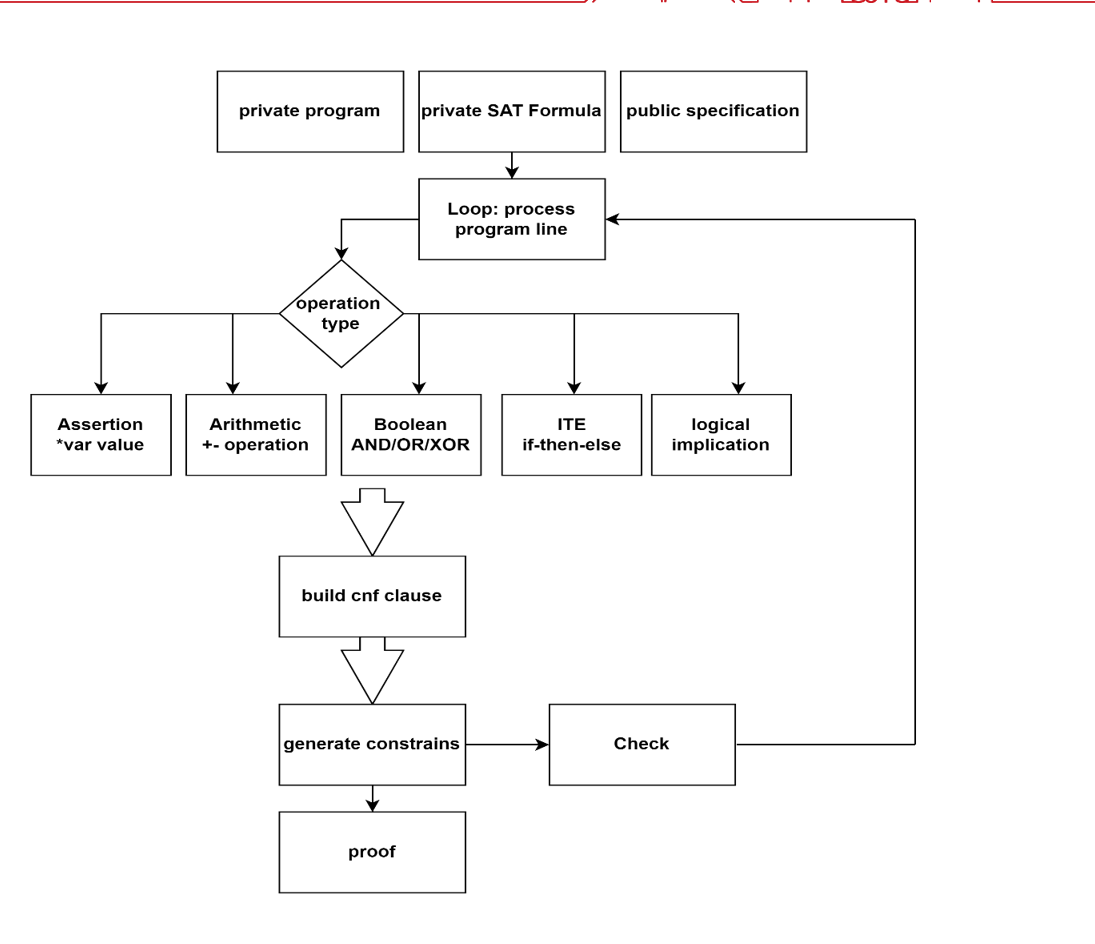
\includegraphics[width=0.85\linewidth]{figures/9.png}
    \bicaption{SSA到SAT转换的zkWASM实现流程}{zkWASM implementation flow for SSA-to-SAT transformation}
    \label{fig:ssa-transformation-flow}
\end{figure}

如图\ref{fig:ssa-transformation-flow}所示,SSA到SAT转换系统在zkWASM中的实现流程包含输入处理、操作类型识别、子句构建和约束验证四个核心环节。

图\ref{fig:ssa-transformation-flow}展示了转换系统的完整执行流程。系统接收三类输入:私有程序$P$包含待验证程序的SSA表示,私有SAT公式包含已生成的CNF子句集合,公开规约包含待验证的属性$\phi$和程序规模参数。转换过程通过循环处理程序的每一行语句,根据操作类型分派到相应的编码模块:断言操作直接生成单元子句强制变量为真;算术操作通过位向量编码转换为布尔电路;布尔运算(AND/OR/XOR)应用Tseitin编码生成3个子句;条件表达式(ITE)递归编码三个子表达式并生成9个等价约束;逻辑蕴含转换为析取形式$(¬a \vee b)$。每个操作模块完成子句构建后,将生成的CNF子句传递给约束生成模块,该模块通过zkWASM的\texttt{require}语句验证编码正确性,包括operator constraint检查运算符映射,encoding constraint验证Tseitin等价性,transformation constraint确保变量一致性。约束验证通过后,系统返回循环继续处理下一行,直到所有语句编码完成。最终系统输出零知识证明$\pi$,包含公式承诺、统计信息和满足所有zkWASM约束的执行轨迹。

表\ref{tab:zkwasm-io-ssa}给出zkWASM执行的输入输出规范。

\begin{table}[htbp]
\centering
\bicaption{SSA到SAT转换的zkWASM输入输出规范}{zkWASM I/O specification for SSA-to-SAT}
\label{tab:zkwasm-io-ssa}
\begin{tabular}{llp{7.5cm}}
\toprule
类型 & 可见性 & 内容描述 \\
\midrule
\multicolumn{3}{l}{\textit{输入规范}} \\
私有输入 & 仅证明者 & SSA程序$P$的语句序列和变量依赖关系 \\
私有输入 & 仅证明者 & 编码过程中生成的辅助变量和中间CNF子句 \\
公开输入 & 双方可见 & 属性规约$\phi$的形式化描述 \\
公开输入 & 双方可见 & 程序规模参数$(|V|, |S|, w)$ \\
\midrule
\multicolumn{3}{l}{\textit{输出规范}} \\
私有输出 & 仅证明者 & 完整CNF公式$F = \{C_1, \ldots, C_k\}$ \\
公开输出 & 双方可见 & 公式承诺$\text{com} = \text{Commit}(F, r)$ \\
公开输出 & 双方可见 & 统计信息(子句数$|F|$,辅助变量数) \\
\bottomrule
\end{tabular}
\end{table}

zkWASM通过四类约束确保编码正确性。变量分配约束验证每个$v \in V$恰好分配$w$个布尔变量:
\begin{equation}
\texttt{require}\left(\forall v \in V: |\mathcal{M}[v]| = w \wedge \text{distinct}(\mathcal{M}[v])\right)
\end{equation}

编码规则约束(operator constraint)验证生成的CNF子句符合表\ref{tab:logic-encoding}的Tseitin编码,对每个逻辑运算$z = x \circ y$检查:
\begin{equation}
\texttt{require}\left(F_{\text{gen}}(z, x, y) = F_{\text{std}}(\circ)\right)
\end{equation}
其中$F_{\text{gen}}$为生成的子句,$F_{\text{std}}$为标准Tseitin编码。

Tseitin等价性约束(encoding constraint)验证辅助变量保持逻辑等价,对每个辅助变量$a$表示子表达式$e$:
\begin{equation}
\texttt{require}\left(\forall \alpha: \text{Eval}(a, \alpha) = \text{Eval}(e, \alpha)\right)
\end{equation}

承诺一致性约束验证公式承诺正确绑定到生成的CNF:
\begin{equation}
\texttt{require}\left(\text{Open}(\text{com}, F, r) = \top\right)
\end{equation}

算法复杂度:设程序包含$n$个语句,每个表达式平均$k$个运算符。变量分配$O(|V| \cdot w)$,语句编码$O(n \cdot k)$,总时间复杂度$O(n \cdot k + |V| \cdot w)$。空间复杂度由CNF公式占据,为$O(n \cdot k)$。

\subsection{性质证明}

本节证明基于zkWASM的SSA到SAT转换系统满足零知识证明的三个核心性质:完备性、可靠性和零知识性。

\begin{theorem}[完备性]
若程序$P$满足属性$\phi$,则诚实证明者能够生成被验证者接受的证明。
\end{theorem}

\begin{proof}
若$P \models \phi$,则验证条件$\text{VC}(P, \phi) = \bigwedge_{i} \tau(\sigma_i) \wedge \neg\phi$不可满足。诚实证明者执行算法\ref{alg:ssa-to-sat-zkwasm}:

变量分配阶段为每个变量$v$分配位向量$\mathcal{M}[v]$,zkWASM约束验证位宽正确。语句编码阶段递归编码每个表达式,生成CNF子句。根据Tseitin编码的健全性,生成的子句保持逻辑等价。zkWASM的operator constraint验证运算符正确映射,encoding constraint验证子句符合标准。属性否定阶段对$\phi$编码并否定,由于$P \models \phi$,生成的公式$F$不可满足。
zkWASM约束系统验证编码过程每步正确,诚实证明者的执行满足所有约束,验证者接受证明。
\end{proof}

\begin{theorem}[可靠性]
若程序$P$不满足属性$\phi$,则恶意证明者伪造有效证明的概率可忽略。
\end{theorem}

\begin{proof}
设域大小$|\mathbb{F}_p| = p$。若$P \not\models \phi$,则生成的公式$F$可满足。恶意证明者的攻击向量:

篡改程序:zkWASM要求程序规模与公开参数一致,承诺正确绑定。修改程序导致承诺不匹配,验证失败。

违反编码规则:operator constraint强制运算符按标准Tseitin规则编码。偏离标准编码的子句违反约束,被检测。

破坏等价性:若辅助变量$a$与子表达式$e$不等价,存在赋值使二者求值不同。由Schwartz-Zippel引理,对度数为$d$的多项式,随机点检测不等价的概率为$1 - d/p$。对合理表达式,$d \ll p$,检测概率接近1。

伪造承诺:基于抗碰撞哈希函数的承诺方案,找到碰撞的概率至多$1/p$。

综合上述,恶意证明者成功概率$\epsilon \leq 1/p \approx 2^{-256}$,可忽略。
\end{proof}

\begin{theorem}[零知识性]
zkWASM协议满足计算零知识性:验证者仅获得验证结果,不泄露程序或公式的任何信息。
\end{theorem}

\begin{proof}
构造多项式时间模拟器$\mathcal{S}$,仅知验证结果和公开参数,生成与真实交互计算不可区分的视图。
$\mathcal{S}$随机生成程序$P^{\text{sim}}$满足规模参数,执行编码算法生成公式$F^{\text{sim}}$。计算承诺$\text{com}^{\text{sim}}$,由承诺方案的隐藏性,其分布与真实承诺不可区分。利用底层SNARK的零知识模拟器生成证明$\pi^{\text{sim}}$,无需真实witness。
验证者观察$(公开参数, \text{com}, \pi, 结果)$。由承诺隐藏性和SNARK零知识性,真实视图与模拟视图计算不可区分。协议不泄露私有信息,满足零知识性。
\end{proof}

这三个定理基于Schwartz-Zippel引理和密码学假设,确立了zkWASM实现的转换系统的安全性。

\section{基于zkWASM的符号执行系统}

本节描述基于zkWASM实现的符号执行算法。符号执行通过探索程序的执行路径，生成路径约束（SMT公式），进而通过位分解转换为SAT公式，用于可达性验证和漏洞检测。

\subsection{基于zkWASM的符号执行算法}

算法 \ref{alg:symbolic-simple} 描述了在 zkWASM 中实现的符号执行到 SAT 转换流程。

\begin{algorithm}[H]
\SetAlgoLined
\bicaption{基于 zkWASM 的符号执行算法}{Simplified zkWASM-based Symbolic Execution}
\label{alg:symbolic-simple}
\KwIn{程序 $P$, 位宽 $w$, 深度限制 $D$}
\KwOut{逻辑公式集 $\{F_1, \ldots, F_k\}$}

\tcp{1. 路径探索}
初始化状态集 $W$；
\While{$W$ 不为空}{
    取出状态 $(s, PC, d)$；\texttt{require}($d \leq D$) \tcp*{深度检查}
    \uIf{$s$ 为赋值}{更新变量符号状态并推入 $W$\;}
    \uElseIf{$s$ 为分支}{将满足条件的可行路径约束 $PC'$ 推入 $W$\;}
    \uElseIf{$s$ 为目标}{记录路径约束 $PC$\;}
}

\tcp{2. 位分解转换}
\ForEach{路径约束 $PC$}{
    将变量拆解为 $w$ 位向量，并将算术操作映射为等效逻辑电路\;
    \texttt{require}(电路逻辑与原操作语义一致)\;
    生成逻辑公式 $F$ 并存入结果集\;
}
\KwRet 结果集\;
\end{algorithm}

该算法通过路径搜索与位分解两个环节实现逻辑转化。在探索阶段，算法利用工作列表递归遍历程序分支，并在 zkWASM 深度约束下实时更新变量状态，从而记录下所有可达路径的逻辑组合。随后在转化阶段，算法将这些抽象约束“翻译”为底层比特逻辑，通过将整数变量拆解为位向量并构建等效的逻辑电路，确保生成的数学公式集能精确还原程序的原始执行语义，并最终输出可供验证的 SAT 公式。

\subsection{基于 zkWASM 的符号执行系统实现}

如图\ref{fig:zkwasm-symbolic-arch} 所示，该系统通过 zkWASM 构建了一个隐私保护的证明架构。证明者输入私有数据（程序 $P$ 与符号状态），并结合公开的验证规范，在 zkWASM 约束引擎中完成证明。引擎内部包含算子约束（operator constraint）、编码约束（encoding constraint）及转换约束（transformation constraint），确保从程序逻辑到公式编码的每一步都受到电路规则的硬性审计，最终输出不可伪造的证明承诺（Proof）。

\begin{figure}[htbp]
    \centering
    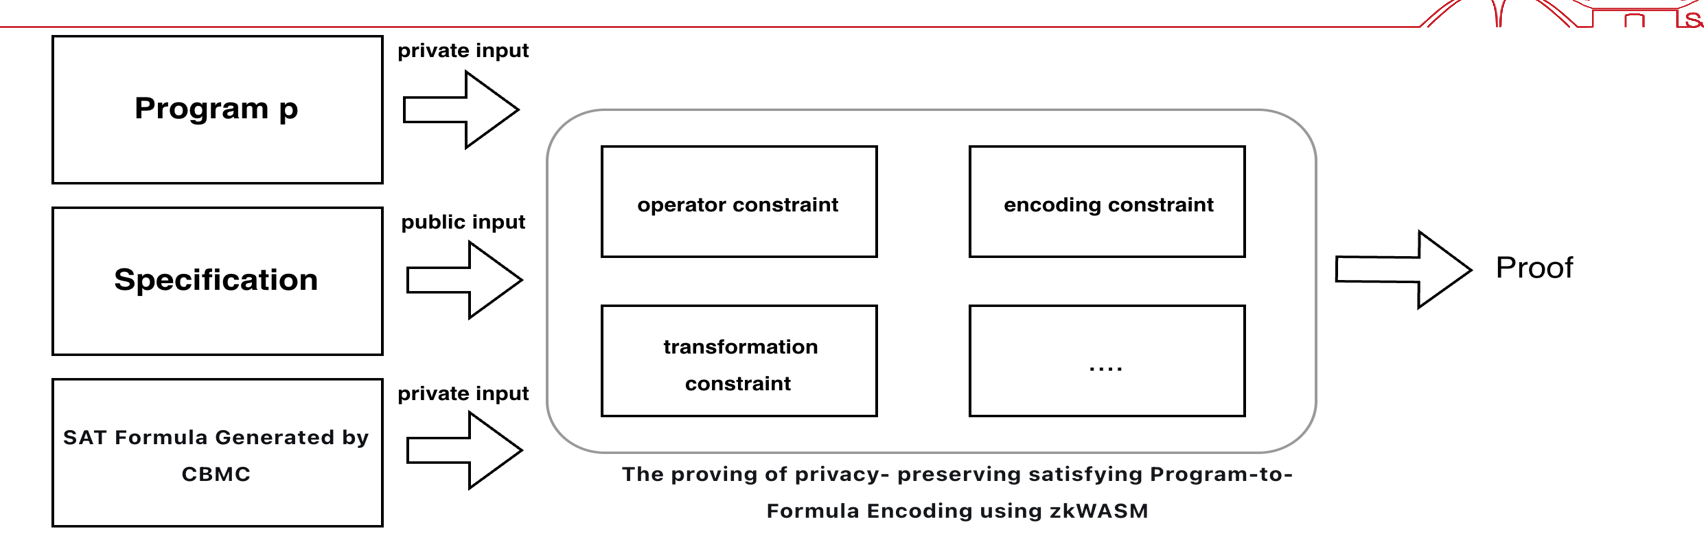
\includegraphics[width=0.85\linewidth]{figures/10.png}
    \bicaption{基于 zkWASM 的符号执行证明架构}{zkWASM-based Symbolic Execution Proving Architecture}
    \label{fig:zkwasm-symbolic-arch}
\end{figure}

表 \ref{tab:zkwasm-io-symbolic} 给出了 zkWASM 执行过程中的输入输出规范。

\begin{table}[htbp]
\centering
\bicaption{符号执行的 zkWASM 输入输出规范}{zkWASM I/O specification for symbolic execution}
\label{tab:zkwasm-io-symbolic}
\begin{tabular}{llp{7.5cm}}
\toprule
类型 & 可见性 & 内容描述 \\
\midrule
\textit{输入规范} & & \\
私有输入 & 仅证明者 & 程序控制流图、符号状态 $\sigma$、工作列表 $W$ \\
公开输入 & 双方可见 & 探索参数 $(D, \text{目标})$ \\
\midrule
\textit{输出规范} & & \\
私有输出 & 仅证明者 & 路径集合、SAT 公式集 \\
公开输出 & 双方可见 & 可达性结果、路径数、证明承诺 \\
\bottomrule
\end{tabular}
\end{table}

zkWASM 通过四类约束确保转换正确性。状态更新约束验证赋值操作后符号状态的一致性：
\begin{equation}
\texttt{require}(\sigma'(v) = \sigma(e))
\end{equation}

路径约束累积验证分支跳转逻辑在路径上的正确叠加：
\begin{equation}
\texttt{require}(PC_{\text{new}} = PC \wedge \sigma(e) \quad \text{或} \quad PC \wedge \neg\sigma(e))
\end{equation}

位表示约束验证整数到二进制位向量映射的数值准确性：
\begin{equation}
\texttt{require}\left(v = \sum_{i=0}^{w-1} b_i \cdot 2^i\right)
\end{equation}

电路等价性约束验证底层的位分解电路是否准确还原了原有的算术或比较操作语义：
\begin{equation}
\texttt{require}(F_{\text{circuit}} \Leftrightarrow \text{原操作})
\end{equation}

在复杂度方面，设有 $B$ 个基本块，分支因子 $b$，深度限制 $D$。系统在最坏情况下需探索 $b^D$ 条路径，每条路径包含 $O(D)$ 个操作，经位分解生成 $O(D \cdot w)$ 个子句。总复杂度为 $O(b^D \cdot D \cdot w)$。

\subsection{性质证明}

本节证明基于 zkWASM 的符号执行转换系统在安全性上满足完备性、可靠性和零知识性。

\begin{theorem}[完备性]
若程序 $P$ 存在深度 $k \leq D$ 的可达路径，则算法必能生成包含该路径的逻辑约束，且 zkWASM 约束验证通过。
\end{theorem}

\begin{proof}
证明基于路径长度归纳。初始状态入队且路径约束为真，满足初始条件。在探索过程中，若当前步骤为赋值，zkWASM 的状态更新约束确保符号值与表达式语义同步；若为分支跳转，由于具体执行路径存在，对应的路径约束（$PC$）在逻辑上必为可满足。由于诚实证明者严格按照算子约束（operator constraint）与编码规则进行转换，生成的位分解电路与原程序操作逻辑等价。因此，算法能够完整记录可达路径并满足所有 zkWASM 校验规则，使验证者接受证明。
\end{proof}

\begin{theorem}[可靠性]
若生成的路径约束可满足，则必存在具体输入使程序执行至目标位置；恶意证明者伪造非法证明的概率在计算上可忽略。
\end{theorem}

\begin{proof}
设有限域大小为 $p$。若路径约束 $PC$ 有解，则可根据该解构造具体输入，使程序在实际运行时沿相同路径到达目标。恶意证明者的攻击行为会被 zkWASM 的约束机制拦截：首先，转换约束（transformation constraint）强制路径累积必须符合程序控制流，防止篡改执行路径；其次，若试图伪造等价电路，根据 Schwartz-Zippel 引理，随机点检测不等价性的概率为 $1 - d/p$，由于 $d \ll p$，检测概率接近 1；最后，伪造承诺需攻破抗碰撞哈希，概率至多 $1/p \approx 2^{-256}$。综上，恶意证明者伪造成功的概率 $\epsilon \leq 1/p$，在安全意义上可忽略。
\end{proof}

\begin{theorem}[零知识性]
zkWASM 协议满足计算零知识性，验证者除可达性结论外，无法获取程序逻辑或路径的具体信息。
\end{theorem}

\begin{proof}
通过构造模拟器 $\mathcal{S}$ 进行证明。$\mathcal{S}$ 在仅知公开参数与验证结果的情况下，随机生成符合规模要求的程序与路径公式。由于 zkWASM 采用的承诺方案具有隐藏性，模拟生成的承诺与真实交互中的承诺在统计分布上不可区分。同时，利用底层 SNARK 的零知识模拟器，可以在无需真实私有 witness（如具体路径路径和变量值）的情况下生成合法的证明凭证。验证者无法区分真实视图与模拟视图，因此协议不泄露任何私有信息。
\end{proof}

上述定理确立了系统在符号执行过程中的安全性，确保了程序验证结论的真实性与隐私性。

\section{基于 HyperPlonk 的 zkWASM 后端优化}

HyperPlonk 是一种基于多线性多项式（Multilinear Polynomials）与和校验协议（Sum-check Protocol）的高性能 zk-SNARK 后端方案。相较于传统基于单变量多项式的 Plonk 协议，HyperPlonk 通过消除对信任设置（Trusted Setup）的依赖，并原生支持高阶定制门（Custom Gates），为 zkWASM 提供了极具扩展性的约束表达框架。其核心优势在于证明者的时间复杂度与约束规模呈严格线性关系，这使得 zkWASM 在处理大规模、复杂的 WebAssembly 指令序列时，能够有效规避因电路规模膨胀而导致的证明生成效率瓶颈，为工业级智能合约的隐私验证奠定了坚实的数学基础。

在系统实现中，该后端优化方案实现了从指令轨迹到零知识证明的高效映射。如图 \ref{fig:hyper-plonk-workflow} 所示，系统首先将 WASM 字节码运行产生的执行轨迹（Execution Trace）映射至 HyperPlonk 约束系统中，利用多线性多项式的分段特性优化高分支逻辑的电路拓扑。

\begin{figure}[htbp]
    \centering
    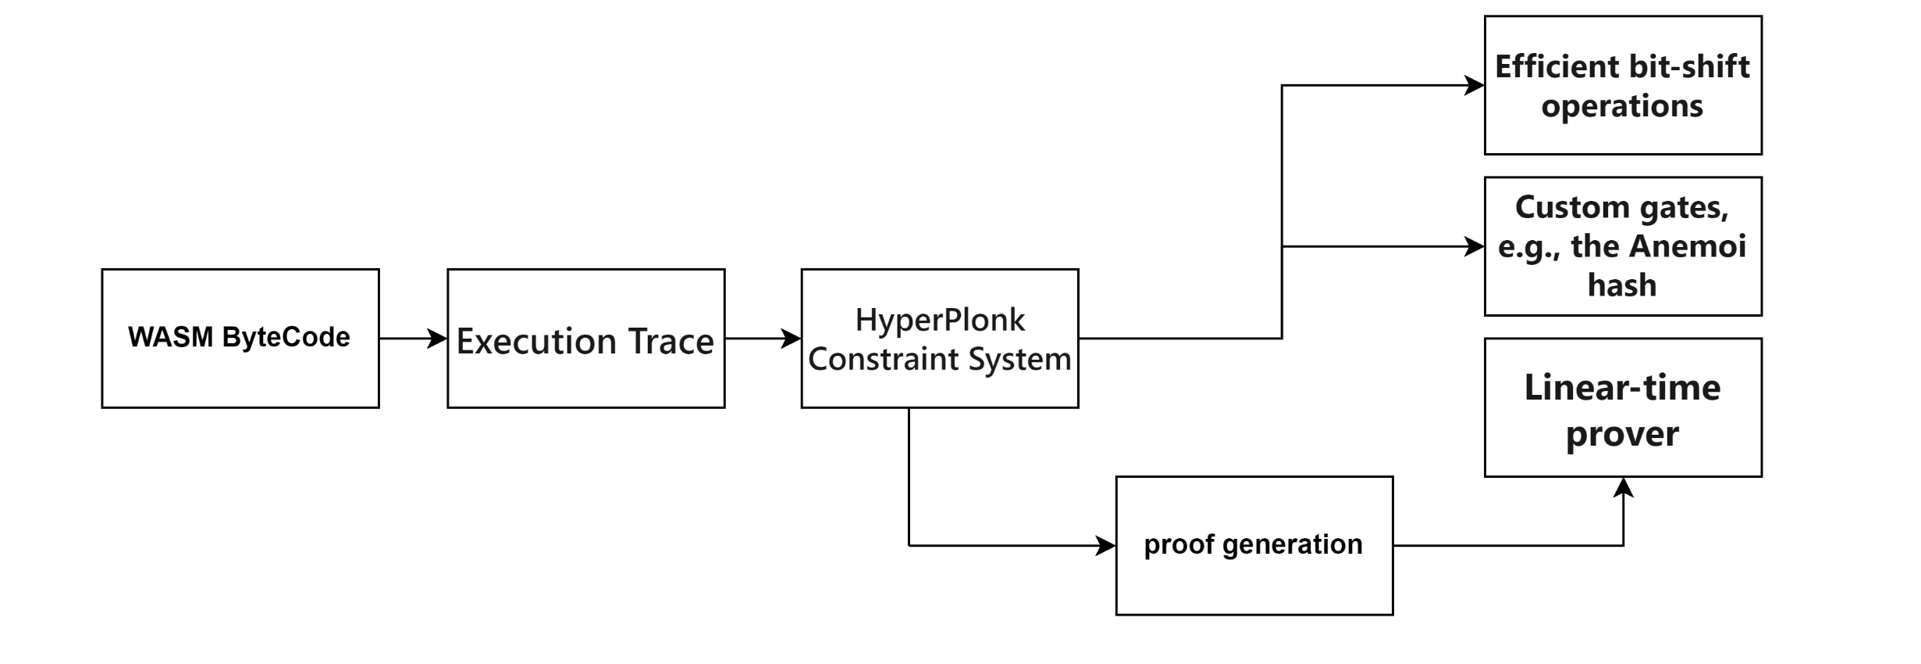
\includegraphics[width=0.9\linewidth]{figures/11.png} % 对应 HyperPlonk 工作流图
    \bicaption{基于 HyperPlonk 的 zkWASM 后端优化工作流}{HyperPlonk-based zkWASM backend optimization workflow}
    \label{fig:hyper-plonk-workflow}
\end{figure}

后端架构针对底层性能瓶颈实施了针对性改进：首先，系统通过“高效位移运算（Efficient bit-shift operations）”优化了 WASM 频繁调用的算术与逻辑位移指令，避免了传统布尔电路逐位展开带来的约束密度剧增；其次，系统集成了 Anemoi 等零知识证明友好型哈希函数的“定制门（Custom gates）”，显著缩减了复杂密码学原语在电路中的计算开销。最终，配合线性时间证明器（Linear-time prover），系统实现了证明生成（Proof generation）耗时与程序执行步数的线性匹配。这种深度的软硬件协同设计，在提升比特位运算性能的同时，确保了 zkWASM 系统在复杂应用场景下的工程实用性与极高性能表现。